\documentclass[11pt,compress,t,notes=noshow, xcolor=table]{beamer}
\usepackage[]{graphicx}\usepackage[]{color}
% maxwidth is the original width if it is less than linewidth
% otherwise use linewidth (to make sure the graphics do not exceed the margin)
\makeatletter
\def\maxwidth{ %
  \ifdim\Gin@nat@width>\linewidth
    \linewidth
  \else
    \Gin@nat@width
  \fi
}
\makeatother

\newcommand{\citebutton}[2]{%
\beamergotobutton{\href{#2}{#1}}%
}

\newcommand{\blu}[1]{\textcolor{blue}{#1}}
\newcommand{\org}[1]{\textcolor{orange}{#1}}
\newcommand{\ques}{\textbf{\textcolor{red}{Question:  }}}
\newcommand{\questionssofar}{\begin{frame}\frametitle{Any questions?}\end{frame}}

\newcommand\warning{%
 \makebox[1.4em][c]{%
 \makebox[0pt][c]{\raisebox{.1em}{\scriptsize!}}%
 \makebox[0pt][c]{\color{red}\normalsize$\bigtriangleup$}}}%

\definecolor{fgcolor}{rgb}{0.345, 0.345, 0.345}
\newcommand{\hlnum}[1]{\textcolor[rgb]{0.686,0.059,0.569}{#1}}%
\newcommand{\hlstr}[1]{\textcolor[rgb]{0.192,0.494,0.8}{#1}}%
\newcommand{\hlcom}[1]{\textcolor[rgb]{0.678,0.584,0.686}{\textit{#1}}}%
\newcommand{\hlopt}[1]{\textcolor[rgb]{0,0,0}{#1}}%
\newcommand{\hlstd}[1]{\textcolor[rgb]{0.345,0.345,0.345}{#1}}%
\newcommand{\hlkwa}[1]{\textcolor[rgb]{0.161,0.373,0.58}{\textbf{#1}}}%
\newcommand{\hlkwb}[1]{\textcolor[rgb]{0.69,0.353,0.396}{#1}}%
\newcommand{\hlkwc}[1]{\textcolor[rgb]{0.333,0.667,0.333}{#1}}%
\newcommand{\hlkwd}[1]{\textcolor[rgb]{0.737,0.353,0.396}{\textbf{#1}}}%
\let\hlipl\hlkwb

\usepackage{framed}
\makeatletter
\newenvironment{kframe}{%
 \def\at@end@of@kframe{}%
 \ifinner\ifhmode%
  \def\at@end@of@kframe{\end{minipage}}%
  \begin{minipage}{\columnwidth}%
 \fi\fi%
 \def\FrameCommand##1{\hskip\@totalleftmargin \hskip-\fboxsep
 \colorbox{shadecolor}{##1}\hskip-\fboxsep
     % There is no \\@totalrightmargin, so:
     \hskip-\linewidth \hskip-\@totalleftmargin \hskip\columnwidth}%
 \MakeFramed {\advance\hsize-\width
   \@totalleftmargin\z@ \linewidth\hsize
   \@setminipage}}%
 {\par\unskip\endMakeFramed%
 \at@end@of@kframe}
\makeatother

\definecolor{shadecolor}{rgb}{.97, .97, .97}
\definecolor{messagecolor}{rgb}{0, 0, 0}
\definecolor{warningcolor}{rgb}{1, 0, 1}
\definecolor{errorcolor}{rgb}{1, 0, 0}
\newenvironment{knitrout}{}{} % an empty environment to be redefined in TeX

\usepackage{alltt}
\newcommand{\SweaveOpts}[1]{}  % do not interfere with LaTeX
\newcommand{\SweaveInput}[1]{} % because they are not real TeX commands
\newcommand{\Sexpr}[1]{}       % will only be parsed by R
\newcommand{\xmark}{\ding{55}}%


\usepackage[english]{babel}
\usepackage[utf8]{inputenc}

\usepackage{dsfont}
\usepackage{verbatim}
\usepackage{amsmath}
\usepackage{amsfonts}
\usepackage{amssymb}
\usepackage{bm}
\usepackage{csquotes}
\usepackage{multirow}
\usepackage{longtable}
\usepackage{booktabs}
\usepackage{enumerate}
\usepackage[absolute,overlay]{textpos}
\usepackage{psfrag}
\usepackage{algorithm}
\usepackage{algpseudocode}
\usepackage{eqnarray}
\usepackage{arydshln}
\usepackage{tabularx}
\usepackage{placeins}
\usepackage{tikz}
\usepackage{setspace}
\usepackage{colortbl}
\usepackage{mathtools}
\usepackage{wrapfig}
\usepackage{bm}
\usepackage{amsmath}
\usepackage{pifont}

\usetikzlibrary{shapes.multipart,shapes,arrows,automata,positioning,calc,chains,trees, shadows}
\tikzset{
  %Define standard arrow tip
  >=stealth',
  %Define style for boxes
  punkt/.style={
    rectangle,
    rounded corners,
    draw=black, very thick,
    text width=6.5em,
    minimum height=2em,
    text centered},
  % Define arrow style
  pil/.style={
    ->,
    thick,
    shorten <=2pt,
    shorten >=2pt,}
}

\tikzstyle{vec}=[draw, rectangle, fill = white, minimum width=5mm, minimum height=1cm, inner sep = 2pt]

\usepackage{subfig}

% Defines macros and environments
\usepackage{../../style/lmu-lecture}


\let\code=\texttt
\let\proglang=\textsf

\setkeys{Gin}{width=0.9\textwidth}

\setbeamertemplate{frametitle}{\expandafter\uppercase\expandafter\insertframetitle}

\usepackage{bbm}
% basic latex stuff
\newcommand{\pkg}[1]{{\fontseries{b}\selectfont #1}} %fontstyle for R packages
\newcommand{\lz}{\vspace{0.5cm}} %vertical space
\newcommand{\dlz}{\vspace{1cm}} %double vertical space
\newcommand{\oneliner}[1] % Oneliner for important statements
{\begin{block}{}\begin{center}\begin{Large}#1\end{Large}\end{center}\end{block}}


%new environments
\newenvironment{vbframe}  %frame with breaks and verbatim
{
 \begin{frame}[containsverbatim,allowframebreaks]
}
{
\end{frame}
}

\newenvironment{vframe}  %frame with verbatim without breaks (to avoid numbering one slided frames)
{
 \begin{frame}[containsverbatim]
}
{
\end{frame}
}

\newenvironment{blocki}[1]   % itemize block
{
 \begin{block}{#1}\begin{itemize}
}
{
\end{itemize}\end{block}
}

\newenvironment{fragileframe}[2]{  %fragile frame with framebreaks
\begin{frame}[allowframebreaks, fragile, environment = fragileframe]
\frametitle{#1}
#2}
{\end{frame}}


\newcommand{\myframe}[2]{  %short for frame with framebreaks
\begin{frame}[allowframebreaks]
\frametitle{#1}
#2
\end{frame}}

\newcommand{\remark}[1]{
  \textbf{Remark:} #1
}


\newenvironment{deleteframe}
{
\begingroup
\usebackgroundtemplate{
\includegraphics[width=\paperwidth,height=\paperheight]{../style/color/red.png}}
 \begin{frame}
}
{
\end{frame}
\endgroup
}
\newenvironment{simplifyframe}
{
\begingroup
\usebackgroundtemplate{
\includegraphics[width=\paperwidth,height=\paperheight]{../style/color/yellow.png}}
 \begin{frame}
}
{
\end{frame}
\endgroup
}\newenvironment{draftframe}
{
\begingroup
\usebackgroundtemplate{
\includegraphics[width=\paperwidth,height=\paperheight]{../style/color/green.jpg}}
 \begin{frame}
}
{
\end{frame}
\endgroup
}
% https://tex.stackexchange.com/a/261480: textcolor that works in mathmode
\makeatletter
\renewcommand*{\@textcolor}[3]{%
  \protect\leavevmode
  \begingroup
    \color#1{#2}#3%
  \endgroup
}
\makeatother





\input{../../latex-math/basic-math.tex}
\input{../../latex-math/basic-ml.tex}

\tikzstyle{squ}=[draw, rectangle, minimum size = 5mm]
\tikzstyle{del}=[squ, fill = white]

%\newcommand{\titlefigure}{figure/word_emb.png}
\newcommand{\learninggoals}{
\item Understand recurent structure of RNNs
\item Learn the different types of RNNs
\item Understand applicability of RNNs}

\title{Advanced NN Architectures}
% \author{}
\institute{\href{https://slds-lmu.github.io/lecture_dl4nlp/}{slds-lmu.github.io/lecture\_dl4nlp}}
\date{}

\begin{document}
\lecturechapter{Recurrent Neural Networks}
\lecture{Deep Learning for NLP}

% ------------------------------------------------------------------------------

\begin{vbframe}{What are RNNs?}

\vfill

\begin{itemize}
	\item Assumption: Text is written sequentially, so our model should read it sequentially
	\item ``RNN'': class of Neural Network architectures that process text sequentially (left-to-right or right-to-left)
	\item Generally speaking:
		\begin{itemize}
			\item Internal ``state'' $\vec h$
			\item RNN consumes one input $\vec x^{(j)}$ per time step $j$
			\item Update function: $\vec h^{(j)} = f(\vec x^{(j)}, \vec h^{({j-1})}; \theta)$
			\begin{itemize}
				\item where parameters $\theta$ are shared across all time steps
			\end{itemize}
		\end{itemize}
\end{itemize}

\vfill

\end{vbframe}

% ------------------------------------------------------------------------------

\begin{vbframe}{Vanilla RNN (1)}

\vfill

\begin{itemize}
	\item Let $\vec x^{(1)} \ldots \vec x^{(J)}$, with $\mathbf{x}^{(j)} \in \mathbb{R}^{d'}$ be our input (e.g., a sequence of $d'$-dimensional word embeddings)
	\item Let $\mathbf{h}^{(0)}  = \{0\}^{d}$ be our initial state
	\item Let $\theta = \{\vec W \in \mathbb{R}^{d \times d'}, \vec V \in \mathbb{R}^{d \times d}, \vec b \in \mathbb{R}^{d}\}$ be our parameters
	\item Then the $j$'th update is defined as:
	$$\vec h^{(j)} = \mathrm{tanh}(\vec W \vec x^{(j)}  + \vec V \vec h^{({j-1})} + \vec b)$$
\end{itemize}

\vfill

\end{vbframe}

% ------------------------------------------------------------------------------

\begin{vbframe}{Vanilla RNN (2)}

\vfill

\begin{itemize}
\item Sentence: ``the cat sat''
\item $(\vec x^{(1)}, \vec x^{(2)}, \vec x^{(3)}) = (\vec x^{(\text{the})}, \vec x^{(\text{cat})}, \vec x^{(\text{sat})})$
$$
\footnotesize
\begin{aligned}
\vec h^{(1)} & = \mathrm{tanh}(\vec W \vec x^{(\text{the})} + \vec V \vec h^{(0)} + \vec b) = \mathrm{tanh}(\vec W \vec x^{(\text{the})} + \vec b) \\
\vec h^{(2)} & = \mathrm{tanh}(\vec W \vec x^{(\text{cat})} + \vec V \vec h^{(1)}+ \vec b) = \mathrm{tanh}(\vec W \vec x^{(\text{cat})} + \vec V \mathrm{tanh}(\vec W \vec x^{(\text{the})} + \vec b) + \vec b) \\
\vec h^{(3)} & = \mathrm{tanh}(\vec W \vec x^{(\text{sat})} + \vec V \vec h^{(2)} + \vec b) = \ldots
\end{aligned}
$$
\item \textcolor{red}{Question:} Which word(s) does $\vec h^{(1)}$ depend on?
\begin{itemize}
\item ``the''
\end{itemize}
\item \textcolor{red}{Question:} Which word(s) does $\vec h^{(2)}$ depend on?
\begin{itemize}
\item ``the cat''
\end{itemize}
\item \textcolor{red}{Question:} Which word(s) does $\vec h^{(3)}$ depend on?
\begin{itemize}
\item ``the cat sat''
\end{itemize}
\end{itemize}

\vfill

\end{vbframe}

% ------------------------------------------------------------------------------

\begin{vbframe}{Vanilla RNN cell}

\vfill

\begin{center}
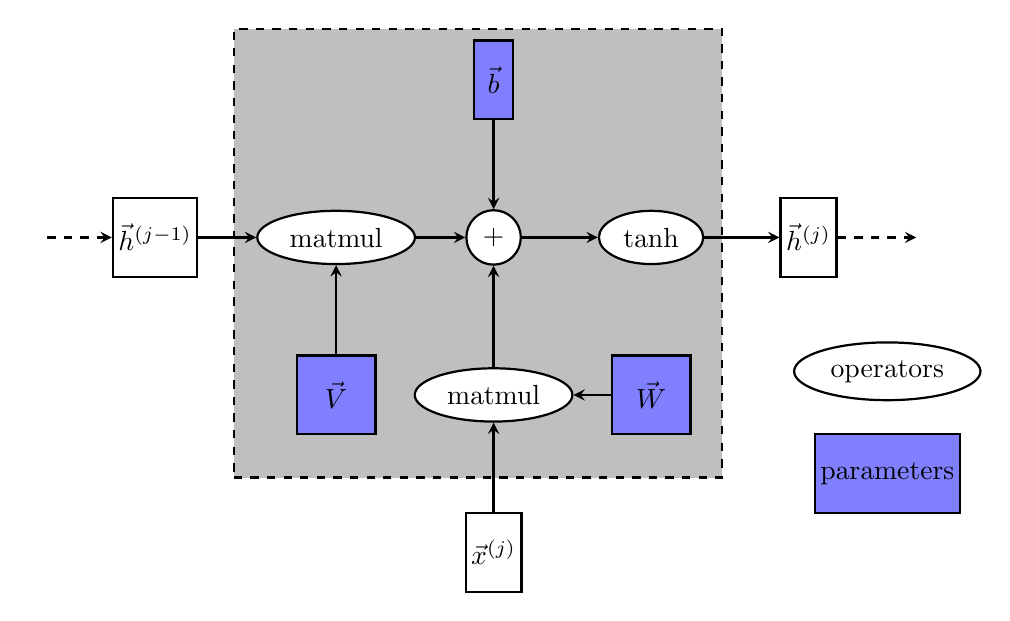
\begin{tikzpicture}[->, >=stealth, thick]
\node at (3.8,3.8) [fill=gray!50, minimum height=5.7cm, minimum width=6.2cm, dashed, draw] {};
\node (hminus) at (-.3,4) [vec] {$\vec h^{(j-1)}$};
\node (x) at (4,0) [vec] {$\vec x^{(j)}$};
\node (h) at (8,4) [vec] {$\vec h^{(j)}$};
\node (dotx) [draw, ellipse, fill=white] at (4,2) {matmul};
\node (doth) [draw, ellipse, fill=white] at (2,4) {matmul};
\node (plus) at (4,4) [draw, circle, fill=white] {$+$};
\node (tanh) at (6,4) [draw, ellipse, fill=white] {$\mathrm{tanh}$};
\node (hright) at (9.5, 4) {};
\node (hleft) at (-1.8, 4) {};
\node (w) at (dotx -| tanh) [vec, minimum size=1cm, fill=blue!50] {$\vec W$};
\node (v) at (dotx -| doth) [vec, minimum size=1cm, fill=blue!50] {$\vec V$};
\node (b) at (4, 6) [vec, fill=blue!50] {$\vec b$};
\draw (x) -- (dotx);
\draw (hminus) -- (doth);
\draw (dotx) -- (plus);
\draw (doth) -- (plus);
\draw (plus) -- (tanh);
\draw (tanh) -- (h);
\draw [dashed] (h) -- (hright);
\draw [dashed] (hleft) -- (hminus);
\draw (b) -- (plus);
\draw (w) -- (dotx);
\draw (v) -- (doth);
\node at (9,2.3) [draw, ellipse] {operators};
\node at (9,1) [vec, fill=blue!50] {parameters};
\end{tikzpicture}
\end{center}

\vfill

\end{vbframe}

% ------------------------------------------------------------------------------

\begin{vbframe}{Example: Binary sentiment classifier}

\vfill

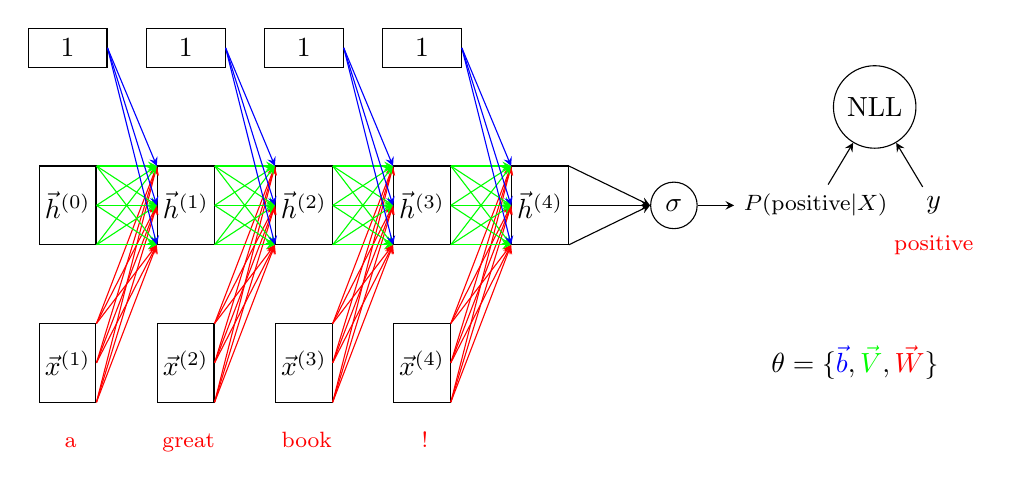
\begin{tikzpicture}
\node [vec] (h0) at (0,2) {$\vec h^{(0)}$};
\foreach \i/\word/\prev in {1/a/0,2/great/1,3/book/2,4/!/3}{
\node [vec] (x\i) at (\i*1.5-1.5, 0) {$\vec x^{(\i)}$};
\node [vec, minimum height=5mm, minimum width=1cm] (b) at (\i*1.5-1.5, 4) {$1$};
\node [vec] (h\i) at (\i*1.5, 2) {$\vec h^{(\i)}$};
\node [text=red] at (\i*1.5-1.5, -1) {\footnotesize \phantom{A}\word\phantom{g}};
\foreach \j in {-5mm,0,5mm}{\foreach \k in {-5mm,0,5mm}{
\draw [->, >=stealth, red] ([yshift=\j]x\i.east) -- ([yshift=\k]h\i.west);}
}
\foreach \j in {-5mm,0,5mm}{\foreach \k in {-5mm,0,5mm}{
\draw [->, >=stealth, green] ([yshift=\j]h\prev.east) -- ([yshift=\k]h\i.west);
}}
\foreach \k in {-5mm,0,5mm}{
\draw [->, >=stealth, blue] (b.east) -- ([yshift=\k]h\i.west);
}
}
\node (ffn) [draw, circle, align=center] at (7.7, 2) {$\sigma$};
\foreach \k in {-5mm,0,5mm}{
\draw [->, >=stealth] ([yshift=\k]h4.east) -- (ffn.west);
}
\node (pred) at (9.5, 2) {\footnotesize $P(\text{positive}|X)$};
\node (y) at (11, 2) {$y$};
\node [text=red] at (11,1.5) {\footnotesize positive};
\draw [->, >=stealth] (ffn) -- (pred);
\node [draw, circle] (loss) at (10.25, 3.25) {NLL};
\draw [->, >=stealth] (pred) -- (loss);
\draw [->, >=stealth] (y) -- (loss);
\node at (10,0) {$\theta = \{\textcolor{blue}{\vec b}, \textcolor{green}{\vec V}, \textcolor{red}{\vec W}\}$};
\end{tikzpicture}
{\footnotesize (Non-linearity omitted for readability.)}

\vfill

\end{vbframe}

% ------------------------------------------------------------------------------

\begin{vbframe}{Backpropagation through time}

\vfill

\begin{itemize}
	\item RNNs are trained via ``backpropagation through time''
	\item To understand how this works, imagine the RNN as a Feed-Forward Net (FFN), whose depth is equal to the sentence length
	\item For now, let's pretend that every time step (every layer) has its own dummy parameters $\theta^{(j)}$, which are identical copies of $\theta$
\end{itemize}

\vfill

\end{vbframe}

% ------------------------------------------------------------------------------

\begin{vbframe}{Vanishing gradients (1)}

\vfill

\begin{itemize}
	\item On long inputs, Vanilla RNNs suffer from ``vanishing'' gradients
	\item Vanishing gradients mean that the impact that an input has on the gradient of the loss becomes smaller when it is further away from the loss in the computation graph.
\end{itemize}

\vfill

\end{vbframe}

% ------------------------------------------------------------------------------

\begin{vbframe}{Vanishing gradients (2)}

\vfill

\begin{itemize}
\item We assume that we have backpropagated the partial derivatives of the loss to $\vec h^{(J)}$:
$$ \frac{\partial L}{\partial \vec h^{(J)}}$$
\item Backpropagate to $\vec h^{(j)}$ via chain rule:
$$
\begin{aligned}
\frac{\partial L}{\partial \vec h^{(j)}} & = \big[\prod_{j'=j+1}^{J} (\frac{\partial \vec h^{(j')}}{\partial \vec h^{(j'-1)}})^T\big] \frac{\partial L}{\partial \vec h^{(J)}} \\
& = \big[\prod_{j'=j+1}^{J} (\frac{\partial \vec V \vec h^{(j'-1)}}{\partial \vec h^{(j'-1)}})^T \frac{\partial \mathrm{tanh}(\vec V \vec h^{(j'-1)} + \ldots)}{\partial \vec V \vec h^{(j'-1)}} \big] \frac{\partial L}{\partial \vec h^{(J)}}
\end{aligned}
$$
\end{itemize}

\vfill

\end{vbframe}

% ------------------------------------------------------------------------------

\begin{vbframe}{Vanishing gradients (3)}

\vfill

$$
\frac{\partial L}{\partial \vec h^{(j)}} = \big[\prod_{j'=j+1}^{J} \textcolor{blue}{(\frac{\partial \vec V \vec h^{(j'-1)}}{\partial \vec h^{(j'-1)}})}^T \textcolor{red}{ \frac{\partial \mathrm{tanh}(\vec V \vec h^{(j'-1)} + \ldots)}{\partial \vec V \vec h^{(j'-1)}}} \big] \frac{\partial L}{\partial \vec h^{(J)}}
$$
\begin{itemize}
	\item What happens to $\frac{\partial L}{\partial \vec h^{(j)}}$ when the distance $J-j$ grows?
		\begin{itemize}
			\item Remember that $\mathrm{tanh}$ is applied elementwise, and that the derivative of $\mathrm{tanh}$ is between 0 an 1. So the \textcolor{red}{red Jacobian matrix} is a diagonal matrix with entries between 0 and 1.
			The product of many such matrices approaches zero.
			\item Furthermore, the \textcolor{blue}{blue Jacobian matrix} is just $\vec V$. When initialized with small enough values, $\prod \vec V$ will approach zero as well.
			\item As a result, $\frac{\partial L}{\partial \vec h^{(j)}}$ approaches zero (``vanishes'')
		\end{itemize}
\end{itemize}

\vfill

\end{vbframe}

% ------------------------------------------------------------------------------

\begin{vbframe}{Vanishing gradients (4)}

\vfill

\begin{itemize}
\item What does this mean?
	\begin{itemize}
		\item Since the ``dummy parameter gradients'' of step $j$, $\nabla_{\theta^{(j)}} L$ are upstream from $\frac{\partial L}{\partial \vec h^{(j)}}$, they approach zero too, i.e., their effect on the ``dummy gradient sum'' is negligible.
		\item This  means that if the words that your RNN should be paying attention to are far from the loss, the network will not (or slowly) adjust its weights to those words
	\end{itemize}
\end{itemize}

\vfill

\end{vbframe}

% ------------------------------------------------------------------------------

\begin{vbframe}{Exploding gradients}

\vfill

\begin{itemize}
	\item So why don't we just use a nonlinearity with a derivative larger than 1, or initialize $\vec V$ differently?
		\begin{itemize}
			\item $||\frac{\partial L}{\partial \vec h^{(j)}}||$ would become very large (``explode''). This is even worse than vanishing gradients, because it leads to non-convergence of gradient descent.
			\item So vanishing gradients is the lesser of two evils.
		\end{itemize}
\end{itemize}

\vfill

\end{vbframe}

% ------------------------------------------------------------------------------

\begin{vbframe}{Long-Short Term Memory Network (1)}

\vfill

\begin{itemize}
	\item Proposed in Hochreiter and Schmidhuber, 1997
	\item Became popular around 2010 for handwriting recognition, speech recognition, and many NLP problems
	\item Addresses vanishing gradients by changing the architecture of the RNN cell
\end{itemize}

\vfill

\end{vbframe}

% ------------------------------------------------------------------------------

\begin{vbframe}{Long-Short Term Memory Network (2)}

\vfill

\begin{itemize}
	\item Two states: $\vec h$ (``short-term memory'') and $\vec c$ (``long-term memory'')
	\item Candidate state $\vec{\bar{h}} \in \mathbb{R}^d$ corresponds to $\vec h$ in the Vanilla RNN
	\item Interactions are mediated by ``gates'' $\in (0, 1)^d$, which apply elementwise:
		\begin{itemize}
			\item Forget gate $\vec f$ decides what information from $\vec c$ should be forgotten
			\item Input gate $\vec i$ decides what information from $\vec {\bar{h}}$ should be added to $\vec c$
			\item Output gate $\vec o$ decides what information from $\vec c$ should be exposed to $\vec h$
		\end{itemize}
	\item Each gate and the candidate state have their own parameters $\theta^{(i)}, \theta^{(f)}, \theta^{(o)}, \theta^{(\bar{h})}$
	\item ``Gradient highway'' from $\vec c^{(j)}$ to $\vec c^{(j-1)}$, with no non-linearities or matrix multiplications
\end{itemize}

\vfill

\end{vbframe}

% ------------------------------------------------------------------------------

\begin{vbframe}{LSTM definition}

\vskip-1mm

\vfill

$$
\begin{aligned}
\vec h^{(0)} & = \vec c^{(0)} = \{0\}^d \\
\vec f^{(j)} & = \sigma(\vec W^{(f)} \vec x^{(j)} + \vec V^{(f)} \vec h^{(j-1)} + \vec b^{(f)}) \\
\vec i^{(j)} & = \sigma(\vec W^{(i)} \vec x^{(j)} + \vec V^{(i)} \vec h^{(j-1)} + \vec b^{(i)}) \\
\vec o^{(j)} & = \sigma(\vec W^{(o)} \vec x^{(j)} + \vec V^{(o)} \vec h^{(j-1)} + \vec b^{(o)}) \\
\vec {\bar{h}}^{(j)} & = \mathrm{tanh}(\vec W^{(\bar{h})} \vec x^{(j)} + \vec V^{(\bar{h})} \vec h^{(j-1)} + \vec b^{(\bar{h})}) \\
\vec c^{(j)} & = \vec f^{(j)} \odot \vec c^{(j-1)} + \vec i^{(j)} \odot \vec {\bar{h}}^{(j)} \\
\vec h^{(j)} &= \vec o^{(j)} \odot \mathrm{tanh}(\vec c^{(j)})
\end{aligned}
$$

\vfill

\end{vbframe}

% ------------------------------------------------------------------------------

\begin{vbframe}{LSTM cell}

\vfill

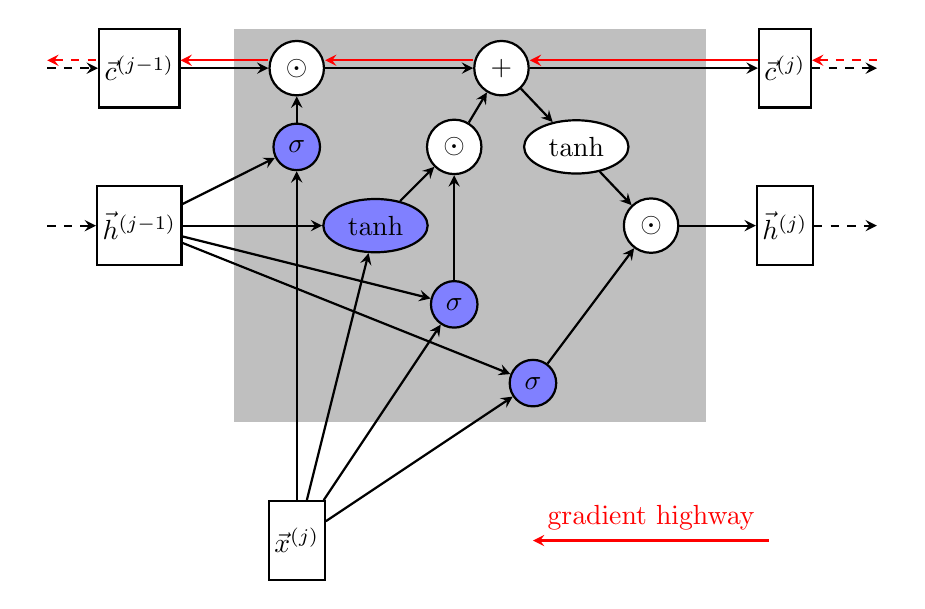
\begin{tikzpicture}[->, >=stealth, thick]
\node at (4.2,2) [fill=gray!50, minimum height=5cm, minimum width=6cm] {};
\node (hminus) at (0,2) [vec] {$\vec h^{(j-1)}$};
\node (cminus) at (0,4) [vec] {$\vec c^{(j-1)}$};
\node (x) at (2,-2) [vec] {$\vec x^{(j)}$};
\node (h) at (8.2,2) [vec] {$\vec h^{(j)}$};
\node (c) at (8.2,4) [vec] {$\vec c^{(j)}$};
\node (i) at (4,1) [draw, circle, fill=blue!50] {$\sigma$};
\node (o) at (5,0) [draw, circle, fill=blue!50] {$\sigma$};
\node (g) at (3,2) [draw, ellipse, fill=blue!50] {$\mathrm{tanh}$};
\node (f) at (2,3) [draw, circle, fill=blue!50] {$\sigma$};
\node (hright) at (9.5, 2) {};
\node (hleft) at (-1.3, 2) {};
\node (cright) at (9.5, 4) {};
\node (cleft) at (-1.3, 4) {};
\foreach \letter in {i,o,f,g}{
\draw (x) -- (\letter);
\draw (hminus) -- (\letter);}
\node [draw, circle, fill=white] (fappli) at (f |- cminus) {$\odot$};
\draw (f) -- (fappli);
\draw (cminus) -- (fappli);
\draw [<-, red] ([yshift=1mm] cminus.east) -- ([yshift=1mm] fappli.west);
\node [draw, circle, fill=white] (iappli) at (i |- f) {$\odot$};
\draw  (i) -- (iappli);
\draw  (g) -- (iappli);
\node [draw, circle, xshift=6mm, fill=white] (plus) at (iappli |- cminus) {$+$};
\draw (iappli) -- (plus);
\draw (fappli) -- (plus);
\draw [<-, red] ([yshift=1mm] fappli.east) -- ([yshift=1mm] plus.west);
\draw (plus) -- (c);
\draw [<-, red] ([yshift=1mm] plus.east) -- ([yshift=1mm] c.west);
\node [draw, circle, xshift=1.5cm, fill=white] (oappli) at (o |-h) {$\odot$};
\node [draw, ellipse, fill=white] at ($(plus)!0.5!(oappli)$) (finaltanh) {$\mathrm{tanh}$};
\draw  (finaltanh) -- (oappli);
\draw (oappli) -- (h);
\draw (o) -- (oappli);
\draw (plus) -- (finaltanh);
\draw [dashed] (h) -- (hright);
\draw [dashed] (c) -- (cright);
\draw [dashed] (hleft) -- (hminus);
\draw [dashed] (cleft) -- (cminus);
\draw [<-, red, dashed] ([yshift=1mm] cleft.east) -- ([yshift=1mm] cminus.west);
\draw [<-, red, dashed] ([yshift=1mm] c.east) -- ([yshift=1mm] cright.west);
\draw [<-, red] (5,-2) --node[midway, above] {gradient highway} (8,-2);
\end{tikzpicture}

\vfill

\end{vbframe}

% ------------------------------------------------------------------------------

\begin{vbframe}{Gated Recurrent Unit (GRU)}

\vfill

\begin{itemize}
	\item Proposed by Cho et al. (2014)
	\item Lightweight alternative to LSTM, with only one state and three sets of parameters
	\item State $\vec h$ is a dynamic ``interpolation'' of long and short term memory
	\item Reset gate $\vec r \in (0,1)^d$ controls what information passes from $\vec h$ to candidate state $\vec {\bar{h}}$
	\item Update gate $\vec z \in (0,1)^d$ interpolates between $\vec h$ and $\vec {\bar{h}}$
	\item Separate set of parameters $\theta^{(r)}, \theta^{(z)}, \theta^{(\bar{h})}$ for each gate and the candidate state.
\end{itemize}

\vfill

\end{vbframe}

% ------------------------------------------------------------------------------

\begin{vbframe}{GRU definition}

\vfill

$$
\begin{aligned}
\vec h^{(0)} & = \{0\}^d \\
\vec r^{(j)} & = \sigma(\vec W^{(r)} \vec x^{(j)} + \vec V^{(r)} \vec h^{(j-1)} + \vec b^{(r)}) \\
\vec z^{(j)} & = \sigma(\vec W^{(z)} \vec x^{(j)} + \vec V^{(z)} \vec h^{(j-1)} + \vec b^{(z)}) \\
\vec {\bar{h}}^{(j)} & = \mathrm{tanh}(\vec W^{(\bar{h})} \vec x^{(j)} + \vec V^{(\bar{h})} (\vec r^{(j)} \odot \vec h^{(j-1)}) + \vec b^{(\bar{h})}) \\
\vec h^{(j)} &= (1-\vec z^{(j)}) \odot \vec h^{(j-1)} + \vec z^{(j)} \odot \vec {\bar{h}}^{(j)} \\
\end{aligned}
$$

\vfill

\end{vbframe}

% ------------------------------------------------------------------------------

\begin{vbframe}{GRU cell}

\vfill

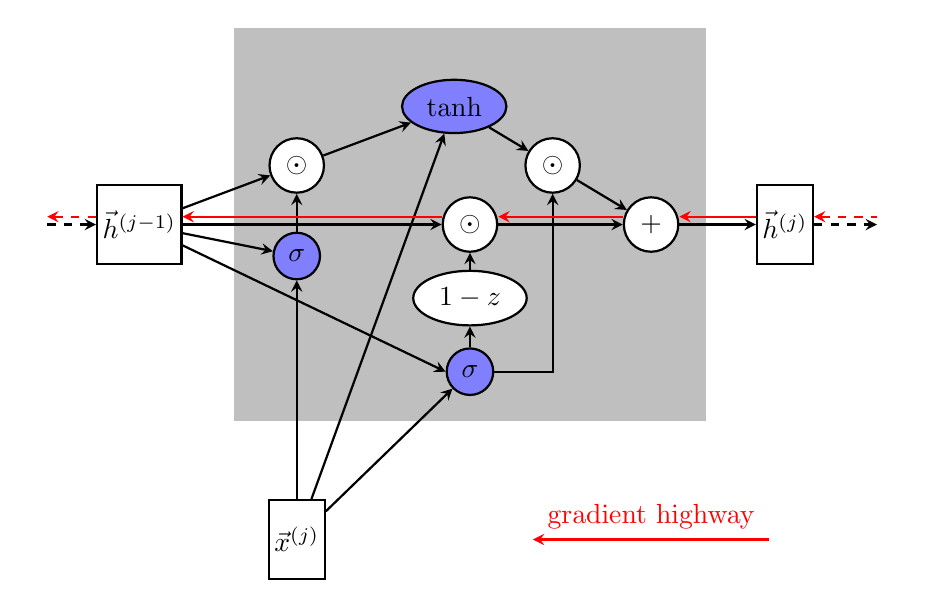
\begin{tikzpicture}[->, >=stealth, thick]
\node at (4.2,2) [fill=gray!50, minimum height=5cm, minimum width=6cm] {};
\node (hminus) at (0,2) [vec] {$\vec h^{(j-1)}$};
\node (x) at (2,-2) [vec] {$\vec x^{(j)}$};
\node (h) at (8.2,2) [vec] {$\vec h^{(j)}$};
\node (r) at (2,1.6) [draw, circle, fill=blue!50] {$\sigma$};
\node (mult2) at (4.2,2) [draw, circle, fill=white] {$\odot$};
\node (z) [draw, circle, below=1.2cm of mult2, fill=blue!50] {$\sigma$};
\node (plus) at (6.5,2) [draw, circle, fill=white] {$+$};
\node (g) at (4,3.5) [draw, ellipse, fill=blue!50] {$\mathrm{tanh}$};
\node at ($(g)!0.5!(hminus)$) [draw, circle, fill=white] (reset) {$\odot$};
\node (mult) at ($(g)!0.5!(plus)$) [draw, circle, fill=white] {$\odot$};
\node (hright) at (9.5, 2) {};
\node (hleft) at (-1.3, 2) {};
\node (zminus) [draw, ellipse, fill=white] at ($(z)!0.5!(mult2)$) {$1-z$};
\draw (zminus) -- (mult2);
\draw (z.east) -- (z.east -| mult.south) -- (mult.south);
\draw  (z) -- (zminus);
\draw  (hminus) -- (mult2);
\draw  (mult2) -- (plus);
\draw (g) -- (mult);
\draw (mult) -- (plus);
\draw (plus) -- (h);
\draw [<-, red, thick] ([yshift=1mm] plus.east) -- ([yshift=1mm] h.west);
\foreach \letter in {z,g,r}{
\draw (x) -- (\letter);}
\draw (hminus) -- (r);
\draw (hminus) -- (z.west);
\draw (hminus) -- (reset);
\draw (r) -- (reset);
\draw (reset) -- (g);
\draw [dashed] (hleft) -- (hminus);
\draw [dashed] (h) -- (hright);
\draw [<-, red, dashed] ([yshift=1mm] h.east) -- ([yshift=1mm] hright.west);
\draw [<-, red, dashed] ([yshift=1mm] hleft.east) -- ([yshift=1mm] hminus.west);
\draw [<-, red] ([yshift=1mm] mult2.east) -- ([yshift=1mm] plus.west);
\draw [<-, red] ([yshift=1mm] hminus.east) -- ([yshift=1mm] mult2.west);
\draw [<-, red] (5,-2) --node[midway, above] {gradient highway} (8,-2);
\end{tikzpicture}

\vfill

\end{vbframe}

% ------------------------------------------------------------------------------

\begin{vbframe}{Vanilla vs. GRU vs. LSTM}

\vfill

\begin{center}
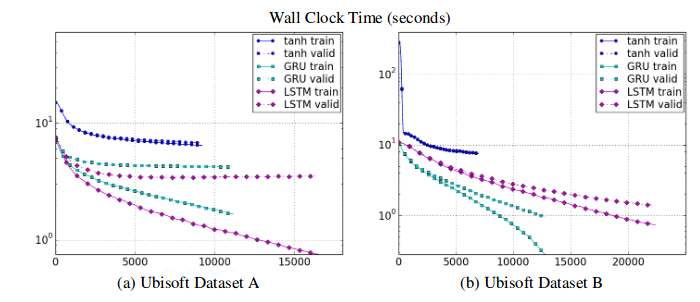
\includegraphics[width=.9\textwidth]{figure/chung}
\end{center}

{\footnotesize Figure from Chung et al. 2014: Empirical Evaluation of Gated Recurrent Neural Networks on Sequence Modeling}

\vfill

\end{vbframe}

% ------------------------------------------------------------------------------

\begin{vbframe}{Tagging (example: Part-Of-Speech)}

\vskip-3mm
\vfill

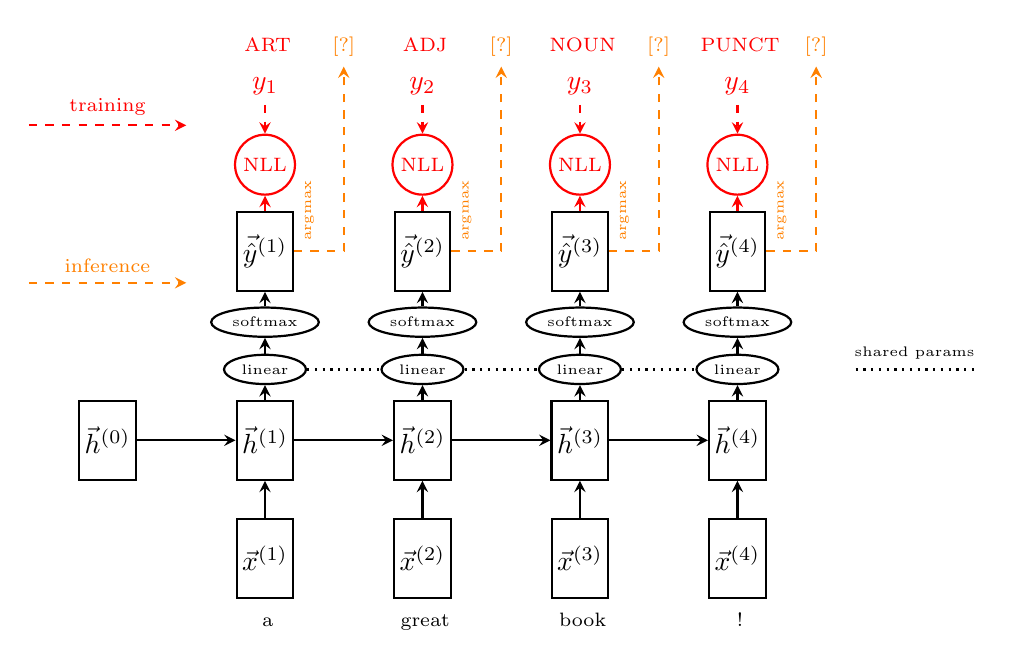
\begin{tikzpicture}[->, >=stealth, thick]
\node [vec] (h0) at (0,2) {$\vec h^{(0)}$};
\foreach \i/\word/\rat in {1/a/ART,2/great/ADJ,3/book/NOUN,4/!/PUNCT}{
\node [vec] (x\i) at (\i*2, .5) {$\vec x^{(\i)}$};
\node [vec] (h\i) at (\i*2, 2) {$\vec h^{(\i)}$};
\node (smax\i) [draw, ellipse, inner sep=2pt] at (\i*2, 3.5) {\tiny softmax};
\node (ffn\i) [draw, ellipse, inner sep=2pt] at (\i*2, 2.9) {\tiny linear};
\node (pred\i) [vec] at (\i*2, 4.4) {$\vec {\hat{y}}^{(\i)}$};
\node (lab\i) at (\i*2, 6.5) [red] {${y}_\i$};
\node (loss\i) [draw, circle, inner sep=2pt, red] at (\i*2, 5.5) {\scriptsize NLL};
\draw (x\i) -- (h\i);
\pgfmathparse{\i-1};
\draw (h\pgfmathresult) -- (h\i);
\draw (h\i) -- (ffn\i);
\draw (ffn\i) -- (smax\i);
\draw (smax\i) -- (pred\i);
\draw (pred\i) [red, dashed] -- (loss\i);
\draw (lab\i) [red, dashed] -- (loss\i);
\node [text=black] at (\i*2,-.3) {\scriptsize \phantom{A}\word\phantom{g}};
\node (tt\i) [orange] at (\i*2+1, 7) {\scriptsize [?]};
\draw [orange, dashed] (pred\i) -- (pred\i -| tt\i) -- (tt\i);
\node [text=red] at (\i*2,7) {\scriptsize \phantom{A}\rat\phantom{g}};
\node [orange, rotate=90, font=\tiny, right=2mm of pred\i] {argmax};
}
\draw [dotted, -] (ffn1) -- (ffn2) -- (ffn3) -- (ffn4);
\draw [dotted, -] (9.5, 2.9) -- node[font=\tiny, midway, above] {shared params} (11, 2.9);
\draw [dashed, orange] (-1, 4) -- node[midway, above, font=\scriptsize] {inference} (1,4);
\draw [dashed, red] (-1, 6) -- node[midway, above, font=\scriptsize] {training} (1,6);
\end{tikzpicture}

\vfill

\end{vbframe}

% ------------------------------------------------------------------------------

\begin{vbframe}{Autoregressive Language Modeling}

\vskip-3mm
\vfill

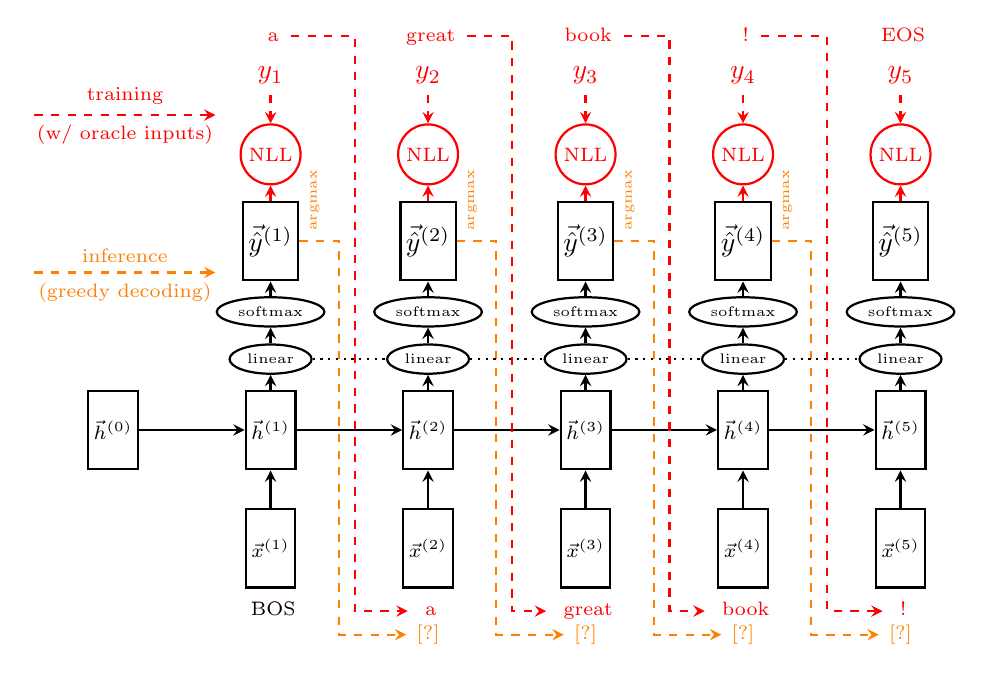
\begin{tikzpicture}[->, thick, >=stealth]
\node [vec] (h0) at (0,2) {\scriptsize $\vec h^{(0)}$};
\foreach \i/\in/\out in {1/BOS/a,2/a/great,3/great/book,4/book/!,5/!/EOS}{
\node (smax\i) [draw, ellipse, inner sep=2pt] at (\i*2, 3.5) {\tiny softmax};
\node (ffn\i) [draw, ellipse, inner sep=2pt] at (\i*2, 2.9) {\tiny linear};
\node (pred\i) [vec] at (\i*2, 4.4) {$\vec {\hat{y}}^{(\i)}$};
\node (lab\i) [red] at (\i*2, 6.5) {${y}_\i$};
\node (loss\i) [draw, circle, inner sep=2pt, red] at (\i*2, 5.5) {\scriptsize NLL};
\node [vec] (x\i) at (\i*2, .5) {\scriptsize $\vec x^{(\i)}$};
\node [vec] (h\i) at (\i*2, 2) {\scriptsize $\vec h^{(\i)}$};
\draw (x\i) -- (h\i);
\pgfmathparse{\i-1};
\draw (h\pgfmathresult) -- (h\i);
\node (in\i) [text=red, inner sep=0pt] at (\i*2,-.3) {\scriptsize \phantom{A}\in\phantom{g}};
\node (out\i) [text=red, inner sep=0pt] at (\i*2,7) {\scriptsize \phantom{A}\out\phantom{g}};
\draw (h\i) -- (ffn\i);
\draw (ffn\i) -- (smax\i);
\draw (smax\i) -- (pred\i);
\draw (pred\i) [red, dashed] -- (loss\i);
\draw (lab\i) [red, dashed]-- (loss\i);
}
\node at (in1) [text=black, fill=white, inner sep=0pt] {\scriptsize \phantom{A}BOS\phantom{g}};

\foreach \j/\t in {2/1,3/2,4/3,5/4}{
\pgfmathparse{\j-1};
\node [right=2mm of pred\t, orange, rotate=90, font=\tiny] {argmax};
\node (argmax\j) [text=orange] at (\j*2,-.6) {\scriptsize [?]};
\node [xshift=-2mm] (pt\j) at ($(ffn\pgfmathresult)!0.5!(ffn\j)$) {};
\node [xshift=-4mm] (px\j) at ($(ffn\pgfmathresult)!0.5!(ffn\j)$) {};
\draw [dashed, red] (out\pgfmathresult) -- (pt\j |- out\pgfmathresult) -- (pt\j |- in\j) -- (in\j);
\draw [dashed, orange] (pred\pgfmathresult) -- (px\j |- pred\pgfmathresult) -- (px\j |- argmax\j) -- (argmax\j);
}
\draw [dotted, -] (ffn1)--(ffn2)--(ffn3)--(ffn4)--(ffn5);
\draw [dashed, orange] (-1, 4) -- node[midway, above, font=\scriptsize] {inference} (1.3,4);
\draw [orange, draw=none] (-1, 4) -- node[midway, below, font=\scriptsize] {(greedy decoding)} (1.3,4);
\draw [dashed, red] (-1, 6) -- node[midway, above, font=\scriptsize] {training} (1.3,6);
\draw [red, draw=none] (-1, 6) -- node[midway, below, font=\scriptsize] {(w/ oracle inputs)} (1.3,6);
\end{tikzpicture}

\vfill

\end{vbframe}

% ------------------------------------------------------------------------------

\begin{vbframe}{Seq-to-seq (Machine Translation)}

\vskip-3mm
\vfill

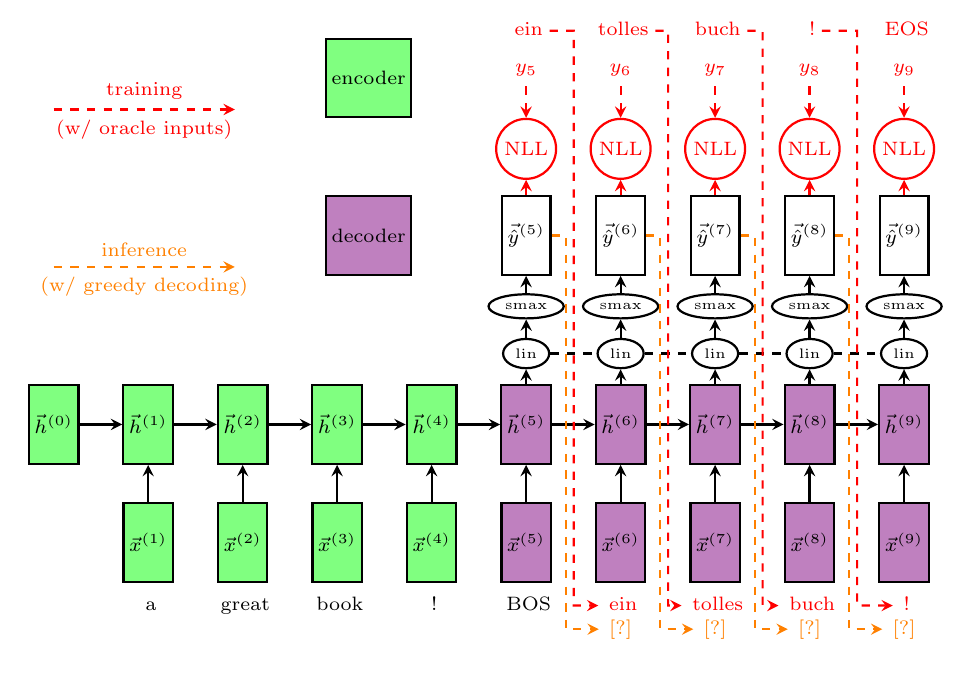
\begin{tikzpicture}[->, thick, >=stealth]
\node [vec, fill=green!50] (h0) at (0,2) {\scriptsize $\vec h^{(0)}$};
\foreach \i/\word/\coll in {1/a/green,2/great/green,3/book/green,4/!/green,5/BOS/violet,6/ein/violet,7/tolles/violet,8/buch/violet,9/!/violet}{
\node [vec, fill=\coll!50] (x\i) at (\i*1.2, .5) {\scriptsize $\vec x^{(\i)}$};
\node [vec, fill=\coll!50] (h\i) at (\i*1.2, 2) {\scriptsize $\vec h^{(\i)}$};
\draw (x\i) -- (h\i);
\pgfmathparse{\i-1};
\draw (h\pgfmathresult) -- (h\i);
}
\foreach \i/\word/\coll in {1/a/green,2/great/green,3/book/green,4/!/green,5/BOS}{
\node (in\i) [text=black, inner sep=-2pt, outer sep=0pt] at (\i*1.2,-.3) {\scriptsize \phantom{A}\word\phantom{g}};
}

\foreach \i/\word/\coll in {6/ein/violet,7/tolles/violet,8/buch/violet,9/!/violet}{
\node (in\i) [text=red, inner sep=-2pt, outer sep=0pt] at (\i*1.2,-.3) {\scriptsize \phantom{A}\word\phantom{g}};
}

\foreach \i/\word in {5/ein,6/tolles,7/buch,8/!,9/EOS}{
\node (smax\i) [draw, ellipse, inner sep=2pt] at (\i*1.2, 3.5) {\tiny smax};
\node (ffn\i) [draw, ellipse, inner sep=2pt] at (\i*1.2, 2.9) {\tiny lin};
\node (pred\i) [vec] at (\i*1.2, 4.4) {\scriptsize $\vec {\hat{y}}^{(\i)}$};
\node (lab\i) [red] at (\i*1.2, 6.5) {\scriptsize ${y}_\i$};
\node (loss\i) [draw, circle, inner sep=2pt, red] at (\i*1.2, 5.5) {\scriptsize NLL};
\node (out\i) [text=red, inner sep=-2pt] at (\i*1.2,7) {\scriptsize \phantom{A}\word\phantom{g}};
\draw  (h\i) -- (ffn\i);
\draw (ffn\i) -- (smax\i);
\draw  (smax\i) -- (pred\i);
\draw (pred\i) [dashed, red] -- (loss\i);
\draw  (lab\i) [dashed, red] -- (loss\i);
}
\draw [dashed, -] (ffn5)--(ffn6)--(ffn7)--(ffn8)--(ffn9);

\draw [dashed, orange] (0, 4) -- node[midway, above, font=\scriptsize] {inference} (2.3,4);
\draw [orange, draw=none] (0, 4) -- node[midway, below, font=\scriptsize] {(w/ greedy decoding)} (2.3,4);
\draw [dashed, red] (0, 6) -- node[midway, above, font=\scriptsize] {training} (2.3,6);
\draw [red, draw=none] (0, 6) -- node[midway, below, font=\scriptsize] {(w/ oracle inputs)} (2.3,6);

\node [vec, fill=green!50] at (4, 6.4) {\scriptsize encoder};
\node [vec, fill=violet!50] at (4, 4.4) {\scriptsize decoder};

\foreach \j/\t in {6/5,7/6,8/7,9/8}{
\pgfmathparse{\j-1};
\node (argmax\j) [text=orange] at (\j*1.2,-.6) {\scriptsize [?]};
\node [xshift=-1.5mm] (pt\j) at ($(ffn\pgfmathresult)!0.5!(ffn\j)$) {};
\node [xshift=-2.5mm] (px\j) at ($(ffn\pgfmathresult)!0.5!(ffn\j)$) {};
\draw [dashed, red] (out\pgfmathresult) -- (pt\j |- out\pgfmathresult) -- (pt\j |- in\j) -- (in\j);
\draw [dashed, orange] (pred\pgfmathresult) -- (px\j |- pred\pgfmathresult) -- (px\j |- argmax\j) -- (argmax\j);
}
\end{tikzpicture}

\vfill

\end{vbframe}

% ------------------------------------------------------------------------------

\begin{vbframe}{Multi-Layer RNNs (1)}

\vfill

\begin{itemize}
\item Stack of several RNNs (Vanilla RNNs, LSTMs, GRUs, etc.)
\item Each RNN in the stack has its own parameters
\item The input vectors of the $l$'th RNN are the hidden states of the $l-1$'th RNN
\item The input vectors to the first RNN are the word embeddings, as usual
\item We can output the hidden states of the last RNN, or a combination (concatenation, average, etc.) of the states of all RNNs.
\end{itemize}

\vfill

\end{vbframe}

% ------------------------------------------------------------------------------

\begin{vbframe}{Multi-Layer RNNs (2)}

\vfill

\begin{center}
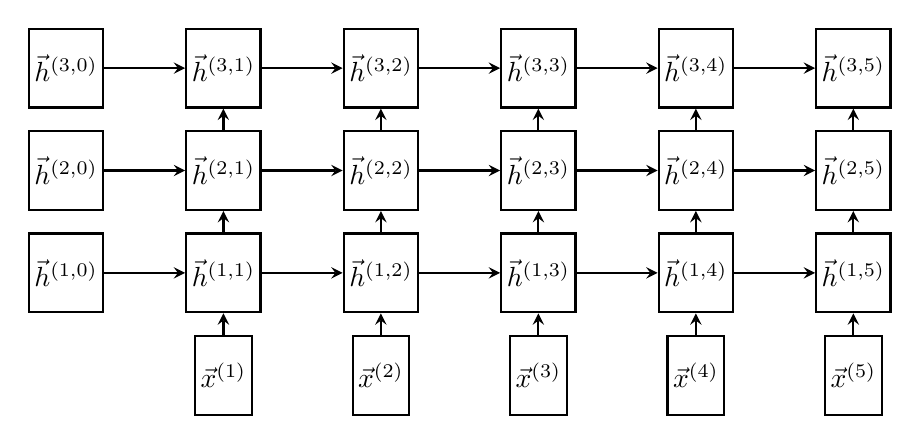
\begin{tikzpicture}[->, thick, >=stealth]
\node (h10) [vec] at (0,1.3) {$\vec h^{(1,0)}$};
\node (h20) [vec] at (0,2.6) {$\vec h^{(2,0)}$};
\node (h30) [vec] at (0,3.9) {$\vec h^{(3,0)}$};
\foreach \i in {1,...,5}{
\node (x\i) [vec] at (\i*2,0) {$\vec x^{(\i)}$};
\node (h1\i) [vec] at (\i*2,1.3) {$\vec h^{(1,\i)}$};
\node (h2\i) [vec] at (\i*2,2.6) {$\vec h^{(2,\i)}$};
\node (h3\i) [vec] at (\i*2,3.9) {$\vec h^{(3,\i)}$};
\pgfmathparse{\i-1};
\draw  (h1\pgfmathresult) -- (h1\i);
\draw  (h2\pgfmathresult) -- (h2\i);
\draw  (h3\pgfmathresult) -- (h3\i);
\draw  (x\i) -- (h1\i);
\draw  (h1\i) -- (h2\i);
\draw  (h2\i) -- (h3\i);
}
\end{tikzpicture}
\end{center}

\vfill

\end{vbframe}

% ------------------------------------------------------------------------------

\begin{vbframe}{Bidirectional RNNs (1)}

\vfill

\begin{itemize}
	\item Two RNNs with separate parameters $\overset{\rightarrow}{\theta}, \overset{\leftarrow}{\theta}$
	\item Let $\vec x^{(1)} \ldots \vec x^{(J)}$ be our input
	\item Let $\overset{\rightarrow}{\vec h}^{(0)} = \overset{\leftarrow}{\vec h}^{(J+1)} = \{0\}^d$ be our initial states.
	\item The forward RNN runs left-to-right over the input:
		$$\overset{\rightarrow}{\vec h}^{(j)} = f(\vec x^{(j)}, \overset{\rightarrow}{\vec h}^{(j-1)}; \overset{\rightarrow}{\theta})$$
	\item The backward RNN runs right-to-left over the input:
		$$\overset{\leftarrow}{\vec h}^{(j)} = f(\vec x^{(j)}, \overset{\leftarrow}{\vec h}^{(j+1)}; \overset{\leftarrow}{\theta})$$
\end{itemize}

\vfill

\end{vbframe}

% ------------------------------------------------------------------------------

\begin{vbframe}{Bidirectional RNNs (2)}

\vfill

\begin{center}
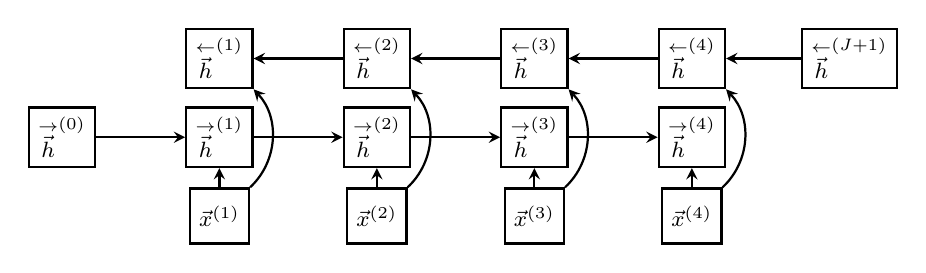
\begin{tikzpicture}[->, thick, >=stealth]
\node (hh10) [font=\footnotesize, minimum height=7mm, draw, rectangle] at (0,1) {$\overset{\rightarrow}{\vec h}^{(0)}$};
\node (hh25) [font=\footnotesize, minimum height=7mm, draw, rectangle] at (10,2) {$\overset{\leftarrow}{\vec h}^{(J+1)}$};

\foreach \i/\j in {1,...,4}{
\node (xx\i) [font=\footnotesize, minimum height=7mm, draw, rectangle] at (\i*2,0) {$\vec x^{(\i)}$};
\node (hh1\i) [font=\footnotesize, minimum height=7mm, draw, rectangle] at (\i*2,1) {$\overset{\rightarrow}{\vec h}^{(\i)}$};
\node (hh2\i) [font=\footnotesize, minimum height=7mm, draw, rectangle] at (\i*2,2) {$\overset{\leftarrow}{\vec h}^{(\i)}$};
}
\foreach \i/\j in {1/2,2/3,3/4}{
\draw  (hh1\i.east) to (hh1\j.west);
\draw  [<-] (hh2\i.east) to (hh2\j.west);
\draw  (xx\i.north) to (hh1\i.south);
\draw  [bend right=45] (xx\i.north east) to (hh2\i.south east);
}
\draw  (xx4.north) to (hh14.south);
\draw  [bend right=45] (xx4.north east) to (hh24.south east);

\draw [<-] (hh24.east) to (hh25.west);
\draw (hh10.east) to (hh11.west);
\end{tikzpicture}
\end{center}

\vfill

\end{vbframe}

% ------------------------------------------------------------------------------

\begin{vbframe}{Bidirectional RNNs (3)}

\vfill

\begin{itemize}
	\item The bidirectional RNN yields two sequences of hidden states:
	$$(\overset{\rightarrow}{\vec h}^{(1)} \ldots \overset{\rightarrow}{\vec h}^{(J)}), (\overset{\leftarrow}{\vec h}^{(1)} \ldots \overset{\leftarrow}{\vec h}^{(J)})$$
	\item \textcolor{red}{Question:} If we are dealing with a sentence classification task, which states should we use to represent the sentence?
		\begin{itemize}
			\item Concatenate $[\overset{\rightarrow}{\vec h}^{(J)};\overset{\leftarrow}{\vec h}^{(1)}]$, because they have ``seen'' the entire sentence
		\end{itemize}
	\item For tagging task, represent the $j$'th word as $[\overset{\rightarrow}{\vec h}^{(j)};\overset{\leftarrow}{\vec h}^{(j)}]$
\end{itemize}

\vfill

\end{vbframe}

% ------------------------------------------------------------------------------

\begin{vbframe}{Bidirectional RNNs (4)}

\vfill

\begin{itemize}
	\item \textcolor{red}{Question:} Can we use a bidirectional RNN for autoregressive language modeling?
		\begin{itemize}
			\item No. In autoregressive language modeling, future inputs must be unknown to the model (since we want to learn to predict them).
			\item We could train two separate autoregressive RNNs (one per direction), but we cannot combine their hidden states before making a prediction
		\end{itemize}
	\item In sequence-to-sequence (e.g., Machine Translation), the encoder can be bidirectional, but the decoder cannot (same reason)
\end{itemize}

\vfill

\end{vbframe}

% ------------------------------------------------------------------------------

\endlecture
\end{document}
